\documentclass[12pt,preprint]{aastex}
\usepackage{url}
\usepackage{natbib}
\usepackage{graphicx}
\usepackage{subfig}
%\usepackage{algorithmic}
\usepackage{appendix}
\usepackage{gensymb}
\usepackage{amsmath}
\usepackage{algpseudocode}

%\usepackage{fixltx2e}



%%%%%%%%%%%%%%%%%%%%%%%%%%%%%%%%%%%%%%%%%%%%%%%%%%%%
%%% author-defined commands
\newcommand\x         {\hbox{$\times$}}
\def\mic              {\hbox{$\mu{\rm m}$}}
\def\about            {\hbox{$\sim$}}
\def\Mo               {\hbox{$M_{\odot}$}}
\def\Lo               {\hbox{$L_{\odot}$}}

%\captionsetup[figure]{labelformat=simple}
%%%%%%%%%%%%%%%%%%%%%%%%%%%%%%%%%%%%%%%%%%%%%%%%%%%%

% Abstract




\begin{document}

\title{Moving Object Pipeline System Design}

\author{Jonathan Myers, Lynne Jones, Tim Axelrod}

\begin{abstract}

The Moving Object Pipeline System (MOPS) has two responsibilities
within LSST Data Management.  First, it is responsible for generating
and managing the \textbf{Moving Object} data products.  The Moving
Objects are identified solar system objects with associated Keplerian
orbits, errors, and detected sources associated with those solar
system objects.  The second responsibility of the MOPS is to predict
future locations of moving objects in incoming images so that their
sources may be associated with known objects; this will reduce the
number of transient detections and prevent Alert Generation on
detections of known Solar System objects.  

\end{abstract}

\tableofcontents


\section{System Design and Responsibilities}

The Moving Object Pipeline System has two main responsibilities: the
generation and maintenance of the Moving Object database, and the
prediction of known object locations which are sent to the Association
Pipeline to prevent unneccessary alerts.  The MOPS has been broken
into two components, colloquially known as ``DayMOPS'' and ``NightMOPS.''
 

\begin{figure}[!ht]
\centering
  \includegraphics[width=13cm]{illustrations/mopsWithinLsst.png}
\caption{ Data flow from the camera through DayMOPS to the Science
  Users and Alert Generation.  DayMOPS will build and maintain the
  Moving Objects table, NightMOPS will use the Moving Objects table to
  communicate with the Assocation Pipeline.  }
\label{mopsWithinLsst}
\end{figure}


``DayMOPS,'' so called because it processes data acquired from the
previous night in a large batch operation, is responsible for
discovering new Moving Objects in newly-acquired data, searching old
data for detections of new objects, and updating the Moving Objects
table to reflect newly-acquired data. It is also responsible for
periodically cleaning and refining the contents of the Moving Objects
table.  ``NightMOPS'' is responsible for projecting the locations of known
Moving Objects in upcoming images as they are announced during
night-time operations.  

The relationship between DayMOPS, NightMOPS and the neighboring
components of the LSST Data Management system is illustrated in
figure \ref{mopsWithinLsst}.

\subsection{DayMOPS: Discovering and Managing Moving Objects}

% Illustration of DayMOPS

% sky-plane vs. orbit-space illustration

The DayMOPS is responsible for discovering moving objects in source
catalogs.  The task of discovering unknown asteroids has a very
lengthy history, involving human, electronic, and computerized actors.

From the beginning the primary detectable feature of an asteroid is
it's motion across the sky as time progresses -- which makes the
underlying orbital parameters of critical relevance to the continued
tracking of the object.  The first asteroid, Ceres, was visually
detected by Piazzi \citep{1802QB378.C4B6.....} through its motions
against the background star as he attempted to verify the position of
a star in a published catalog.  Without knowing how orbits were
goverened, Piazzi's initial tracking effort involved constant repeated
night-to-night observations which he was only able to maintain for a
limited time due to his health and the motion of the asteroid into the
daytime sky.  It fell to Carl Friedrich Gauss to develop his method of
orbit determination before Ceres could be recovered again thus firmly
establishing the mathematics of orbits as a required prerequisite.

Optical observations had their limitations, however, and the archival
record created by the application of photography to observations was
of critical importance to scientific demands of repeatability.  The
first photographic discovery of an asteroid, (323) Brucia, was by Max
Wolf in 1891 \citep{1892AN....129..337W} as he recognized the
non-sidereal rate trails on his photographs for the asteroids they
were.  Wolf became a prolific discoverer of asteroids (almost 250
total) through photography and as such developed the standard
detection technique used for the next century.

Photographic sensitivity is determined to a large part through
exposure time and asteroid motion to first order is a function of its
distance so two main types of photographic survey methodology were
used.  Surveys looking for closeby and fast near-Earth asteroids (like
those of \cite{1988NASTM4041...52S}) used non-sidereal trailed motions
and generally shorter exposure times.  A discovered trail of any
length in the and image developed in an observatory darkroom would
lead to additional exposures of the asteroid being quickly acquired
and the data required to secure the orbit.  The second technique,
useful for very slow moving asteroids that did not appear as a trailed
images was to take several exposures and then manually alternate
between them rapidly, thus depending on the well-developed human
motion sense to discover the moving asteroids.  Machines were built
for this purpose, such as the blink comparator.  Besides its use for
stellar proper motions, this technique's most well known success was
in the discovery of Pluto by Tombaugh \citep{1960S&T....19..264T}.
The blink comparator was useful for scientific studies of asteroids in
the main asteroid belt such as the seminal Palomar-Leiden survey
\citep{1970A&AS....2..339V}.  Keeping the exposure times short was
important to keep the asteroid images starlike so their isophotal
diameter could be used inaccurate brightness calibration.  This
allowed for the rapid discovery of asteroids for the time: 2400
discoveries in 11 nights of observation.

The advent of the CCD was applied to asteroids early, with the long
readout times (and consequential 50\% duty cycle) minimized through
the process of drift scannings.  Gehrels and the Spacewatch Project
\citep{1990ASPC....8...51G} pioneered the use of CCD's in the
detection of asteroids, making the first CCD detection of the
near-Earth asteroid 1989 UP and the first discovery as well (1990 SS).
Spacewatch went on to built an advanced real time asteroid motion
detection program, MODP \citep{1991AJ....101.1518R}.  Drift scanning
was made unnecessary by the advent of large format cameras used in a
step-and-stare mode such as that of the NEAT project
\citep{1999AJ....117.1616P}.  With the introduction of custom
frame-transfer CCD's and high-capacity computer processing, the LINEAR
project \citep{2000Icar..148...21S} and the Catalina Sky Survey
\citep{2007IAUS..236..323L} were able to progress handily towards the
Spaceguard goal.

As with photography, there are multiple techniques which can be
applied to CCD images to discover their asteroids.  Most asteroid
detection software uses a "moving target indicator" approach in that
CCD images are searched automatically for their objects who are then
compiled as a detection list.  By filtering out objects which did not
move and searching for asteroid-like motions in the unmatched lists,
motion candidates are created.  However, a more exotic approach called
Matched Filter Processing \citep{2005AJ....130.1951G} can be applied
that has several advantages.  Images are coadded rapidly along
hypothesized motion vectors.  If the flux of an object appears to grow
after coaddition, it becomes a candidate moving object with the motion
vector already determined.  This approach becomes computationally
expensive with a large number of possible motion vectors but has the
advantage of being able to detect fainter objects in the same set of
images compared to the moving target indicator approach.  It has been
used successfully in searches for distant objects such as those in the
Kuiper Belt \citep{BG, MB} and has been used to do NEA searches over
large portions of the sky where the asteroid is uncertain but has a
relatively small range of possible velocities
\citep{2005AJ....130.1951G}.

The advent of large-format all sky surveys have radically changed the
detection requirements both in terms of techniques for imagery and
software...  heheheh, all yours Jon.  I could only make mistakes in
this part of the discussion.


The design of the LSST DayMOPS is based on the PanSTARRS Moving Object
Pipeline System \citep{psMOPSDesign}.  The approach used here is to
first find sets of detections with sky-plane paths consistent with
asteroid behaviour; these sets of detections and their fitted paths
are called \textbf{tracks}.  A set of algorithms for the discovery of
sky-plane tracks in dense data are presented in
\citet{Kubica:2005:MTA:1081870.1081889}; these algorithms are the
basis of the linking methods for the current LSST DayMOPS.


%% TBD: it would be really nice to have some illustrations here
%% showing detections of an object, and possibly tracklets and tracks
%% as well

The tracking methods used are based on a tiered approach; first two or
more detections from a single night are linked into
\textbf{tracklets}, which represent a hypothetical object and a linear
approximation of its sky-plane motion.  These tracklets are later
joined into larger tracks. Because of the increasing complexity of
sky-plane motion over time, we are generally interested in tracks
which span no more than 15-30 days of observation time.

The PanSTARRS MOPS uses a fairly loose and generous approximation of
asteroid motion.  This allows for many mislinkages or \textbf{false
  tracks}, combining detections which are not attributable to the same
source, but virtually all objects for which a true (correctly-linked)
track could be generated will get some correct track.  With LSST's
expected density of detections, we found that this glut of false
tracks was generally too painful.  As a result, our methods diverge
from those of PanSTARRS as we introduce some more strict filters on
tracks, reducing the number of mislinkages at the expense of
potentially missing some true tracks.  The algorithms, their
implementations, the additional filters, and their behaviors are
presented thoroughly in Chapter \ref{linking}.

Once tracks are discovered, they are sent to the Orbit Determination
phase. The Orbit Determination phase takes these sets of sky-plane
detections and attempts to find a Keplerian orbit which could generate
the detections.  This orbit is further refined, and error bounds are
established, using differential correction.  Orbit Determination will
reject many tracks as false, but should successfully find precise
orbits for virtually all correctly linked tracks.  Several methods for
performing this task are known, and several have open-source implementations
available to LSST \citep{Milani04orbitdetermination},
\citep{Milani2006}, \citep{OpenOrb2009}, \citep{granvik_thesis}.  The
orbits discovered by Orbit Determination, and the detections present
in the track associated with each orbit, are used to generate new
Moving Objects.

\begin{figure}[h]
\begin{center}
  \includegraphics[width=11cm]{illustrations/mopsDiagram.png}
\end{center}
\caption{ Data flows into the DayMOPS pipeline and results in
  modifications of the Moving Objects table in a variety of ways,
  including attribution to known objects, a multi-stage pipeline for
  the discovery of new objects, and periodic refinements of the Moving
  Object table, such as possible merges of redundant objects or
  removal of false orbits. }
\label{mopsDiagram}
\end{figure}



The DayMOPS is expected to perform several additional tasks to manage
and improve the Moving Objects table over time.  Attribution is the
process of identifying known objects in incoming data and adding those
detections to the correct Moving Object, in a process called
Attribution. Similarly, Precovery is the recovery of known,
unattributed detections associated with a newly-discovered Moving
Object.  Another refinement is the merging of potentially redundant
Moving Objects.  The complete set of DayMOPS tasks and their data
flows are illustrated in figure \ref{mopsDiagram}.






\section{DayMOPS}
\label{linking}

\subsection{Approximate Models of Asteroid Motion}
Because of the complexity of the full heliocentric orbital
approximation of asteroid motion, DayMOPS uses simplified models based
on sky-plane motion of asteroid behavior.  


\subsubsection{Real Heliocentric Orbits}
Heliocentric orbits describe an orbit around the Sun.  Generally,
asteroids, planets and other solar system objects follow elliptical
paths, centered on the Sun.  These paths are described (in general
practice as well as the LSST Moving Objects catalog) with a Kepler
orbit, which describes an ellipse using six parameters. 

For purposes of DayMOPS and NightMOPS, we assume that a well-fitted
Kepler orbit should be sufficient to predict the location of an object
well into the future or past.  

\textbf{BD: Illustration of a Kepler orbit - Wikipedia has a good one.}



\subsubsection{Linear and Quadratic Models}
In order to discover and identify new objects, astronomers have
traditionally used sky-plane approximations to predict and model the
behavior of solar system objects for which a true orbit is not yet
known.  As a general rule of thumb, objects are said to move linearly
(with a more or less fixed velocity) in RA and Dec over the course of
a single night and quadratically (having velocity and some
acceleration) in RA and Dec over the course of a month.  These are, of
course, approximations, and linear and quadratic fits will inevitably
contain some error.

Given many detections which may or may not be attributable to one or
more asteroids, these approximations are used to help determine which
detections could plausibly be linked (that is, which detections could
be attributable to the same object).  If several detections over the
course of a single night do not follow a roughly linear path, we trust
that they could not have been attributable to the same object; if
several detections over the course of a month do not follow a roughly
quadratic path, we will trust that they could not be attributable to
the same object.  By ignoring the obviously implausible linkages, we
significantly reduce the number of hypothetical linkages we must
investigate.

Of course, since these are merely approximations, it is almost
inevitable that some correct linkages will be rejected.  In
particular, near-Earth-objects (NEOs) may exhibit sky-plane behaviour
not consistent with these rules of thumb.

\textbf{TBD: Put Yusra's findings here as well}

\subsubsection{Higher-order Sky-Plane Models}
\textbf{TBD: Tim's methods go here - the assumed topocentric distance, topocentric correction, higher-order fits}

\subsection{The Linking Pipeline}
\textbf{TBD: Add an illustration of the various stages and a short piece of
introductory text.  Also perhaps useful: show one object's detections and its various states of linkage. (detections, tracklets, merged tracklets, track(s))}

The LSST DayMOPS system is responsible for finding previously unknown
moving objects in a set of detections.  It takes as input a set of
DiaSource detections with unknown origin.  At output, it should
identify orbits and associated detections for newly-discovered objects
found in the set of input detections.  

The DayMOPS system achieves this through a pipeline approach, building
increasingly sophisticated linkages at each step.  A linkage between a
set of detections represents the hypothesis that these detections
\textit{may} be attributable to the same object.  Unattributed
detections are first linked into nightly linear \textbf{tracklets}.
These tracklets are sets of two or more detections which are roughly
colinear, and have an associated initial sky-plane position and
velocity.  These tracklets are passed forward are passed forward to be
linked into quadratic \textbf{tracks}, each of which contains several
tracklets from multiple nights.  To handle the often large number of
mislinked tracks, a higher-order model is fit the to the detections in
each track and and used to filter them more aggressively.  Those
tracks which survive the filtering are then sent to a full orbit
fitting tool, which should authoritatively reject mislinked sets of
detections and find preliminary orbits associated with
correctly-linked tracks.

Note that tracklets and tracks represent hypothetical linkages, many
of which may be correct.  A single detection may exist in several
tracklets and/or several tracks.  A given tracklet may be found in
multiple tracks.  Some detections may never be linked into any
tracklet; some tracklets will never be linked into any track.  The
DayMOPS system is built using methods and algorithms intended to
efficiently find plausible hypothetical linkages without wasting much
computational time or storage on finding unlikely linkages.

\subsection{Building Tracklets}

\textbf{ possible illustration: show Dec/time for two images, then tracklets in Dec/time}

\textbf{Tracklets} are linkages between DiaSource detections occuring
within the same night. By creating tracklets, DayMOPS can find
sky-plane position and velocity estimates for sets of detections which
may belong to the same solar system objects.  The use of tracklets
also simplifies the downstream work of track generation, which
attempts to find sets of detections with a good
position/velocity/acceleration fit on the sky-plane; since tracklets
have known position and velocity, the track generation phase needs
only to find those tracklets compatible within some acceleration
factor.

Correctly-linked tracklets from a given object are needed to generate
a good track for that object and eventually discover its orbit.
However, if these useful tracklets are too deeply buried among very
large numbers of other tracklets, then the job of tracklet linking
will become extremely slow and expensive.  Generally, these other,
unwanted tracklets are false tracklets (mislinkages between detections
not attributable to the same object), though in special conditions
large numbers of correctly-linked but redundant tracklets can cause
pain as well (this will discussed in \ref{collapseTracklets}).

In order to ensure that tracklet-generating images are acquired, it is
necessary to ensure that fields of the sky are visited two or more
times within an accepted time period each night. To constrain the
number of tracklets, we impose a maximum apparent velocity on the
tracklets, and also require that sky fields be revisited within a
fairly short time period ($\leq 90$ minutes is the current rule).
Raising the maximum velocity threshold enables one to find
faster-moving objects, and raising the maximum allowed revisit time
also enables one to generate tracklets in more fields of the sky;
however, increasing either of these thresholds also increases the
search space and can significantly increase the number of mislinked
tracklets, greatly increasing the cost downstream.




\subsubsection{The findTracklets Software}

The process of initial tracklet creation is accomplished by the
findTracklets software.  Later refinement of tracklets is accomplished
by collapseTracklets and additional filters.

\subsubsubsection{Algorithm} 

The findTracklets software is responsible for finding pairs of
detections which occur within a fixed time threshold, and have
apparent velocity below a given threshold.  For a given detection and
a set of image times, one can calculate the maximum distance an object
could have travelled at each time using the velocity limit.  To find
detections with which the query detection could be linked, one can
imagine searching a circular region in the later images based on this
distance.

\begin{figure}[ht!]
  \centering
    \includegraphics[width=6cm]{illustrations/findTracklets-onequery.png}
    \caption{ An example of searching for compatible second endpoints
      for a given detection.  The first detection and each of the
      second endpoints will be used to create a new tracklet.}
\label{findTrackletsIllustrated}
\end{figure}


Fortunately, this can be
accomplished in a fairly straightforward way through the use of
KD-Trees.  KD-Trees are a data structure which allows for quickly and
efficiently performing range searches on points in space
\citep{bentley_kdtrees}.  A KD-Tree-based method for building
tracklets was first contributed by Jeremy Kubica for his PhD thesis
\citep{kubica_thesis}.  For findTracklets, 2-Dimensional KD-Trees are
used, covering the space of (RA, Dec).  Given a detection and trees
containing detections from later images, we can use range searches to
quickly find nearby detections in those later images and use them for
the creation of tracklets.

\begin{figure}[ht!]
\begin{algorithmic}
\REQUIRE $I$ is a set of images, each of which has an associated exposure time and contains a set of detections
\STATE \COMMENT{Create a 2D KD-Tree for each image, holding detections from that image.}
\STATE $T \gets \{\}$
\FOR {$i \in I$}
  \STATE $t \gets$ Make2DTree$(i.detections)$
  \STATE $t.time \gets i.time$
  \STATE $T \gets T \cup \{t\}$
\ENDFOR
\STATE \COMMENT{Use these trees to discover the actual tracklets.}
\STATE $tracklets \gets \{\}$
\FOR {$t_1 \in T$}
  \STATE $later \gets \{t_i \in T : 0 < t_i.time - t_1.time < maxDt\}$
  \FOR{$d \in t_1.detections$}
     \FOR{$t_q \in later$}
 
       \STATE \COMMENT{Use time between images and max velocity to
         calculate the max travel distance}

        \STATE $dt \gets t_q.time - t_1.time$
        \STATE $dd \gets dt * maxV$
        \STATE \COMMENT{Use KD-Tree range search to find detections within max travel distance}
        \STATE $tracklets \gets tracklets \cup t_q.$rangeSearch($d.ra, d.dec, dd$)
     \ENDFOR
   \ENDFOR
\ENDFOR
\RETURN{$tracklets$}
\end{algorithmic}

\caption{Pseudo-code for the findTracklets algorithm.  2D (RA, Dec)
  trees are created for each image; for each detection, later trees
  are searched for nearby detections. }
 \label{findTrackletsAlgorithm}
\end{figure}


Note that because the sky is a sphere, notions of ``distance'' and
``velocity'' can become slightly confusing, especially near the poles.
Fortunately, both the KD-Tree library used and the findTracklets
software are sufficiently clever to use actual great-circle distance
and velocity for their queries, so that tracklets near the poles are
not missed.  The software should also be impervious to wrap-around
errors - objects which move between, say, $359.9 \degree$ in RA and
$.01 \degree$ in RA will be detected.  The Appendix \ref{kdTreeLib}
explains the KD-Tree library used in greater detail.  

\paragraph{Code and Usage}
Aside from the KD-Tree library, findTracklets is implemented by {\tt
  findTracklets.h}, {\tt findTracklets.cc } and a command-line
interface is provided by {\tt findTrackletsMain.cc}.  When calling the
function {\tt findTracklets()} programmatically (e.g. inside an LSST
Pipeline), use an instance of the {\tt findTrackletsConfig} to set the
values of all options (including max velocity and min/max time
threshold as well as others) and pass this to the {\tt
  findTracklets()} function.  See comments in {\tt findTracklets.h}
for documentation on the {\tt findTrackletsConfig} class.  Also see
\ref{largeData} for additional information on output methods.

The command-line {\tt findTracklets} program will take command-line
flags and use them to instantiate a {\tt findTrackletsConfig} which is
then used to call the actual {\tt findTracklets()} function.  Use {\tt
  \$findTracklets -h} for an overview of the options.






%%%%%%%%%%%%%%%%%%%%%%%%%%%%%%%%%%%%%%%%%%%%%%%%%%%%%%%%%%%%%%%%%%5
%% COLLAPSE TRACKLETS
%%%%%%%%%%%%%%%%%%%%%%%%%%%%%%%%%%%%%%%%%%%%%%%%%%%%%%%%%%%%%%%%%%5


\subsection{Improving and Filtering Tracklets} \label{collapseTracklets}
If a field of the sky gets multiple revisits, or more than two visits
within the time window, it is possible that findTracklets will find
more than one true tracklet associated with that object.  This can
generated needless downstream work, because the number of tracklets is
larger, and if the multiple true intra-nightly tracklets are never
linked together, then useful data (additional detections of the
object) can be lost, or may need to be pieced back together later.

In particular, in ``deep drilling'' operations, the telescope will
repeatedly image the same field of sky many times in a short period.
In these fields, the number of tracklets generated for an object will
grow like $O(n^2)$ where $n$ is the number of times the object is
seen, as each possible pair of detections will be linked.  This can
generate a huge number of tracklets, making later work exceptionally,
and needlessly, difficult.

The tracklet improvement and filtering stage attempts to remedy this
problem by joining together colinear 2-detection tracklets into
higher-cardinality (3 detections or more) tracklets.


\paragraph{Special Considerations}
There is a small risk that occasionally, a true 2-detection tracklet
be merged into a larger tracklet which is mislinked.  This is rare, as
it can only occur when a true tracklet is colinear with a mislinked
tracklet, but it is not strictly impossible.



\subsubsection{The collapseTracklets Software} 

The tracklet refinement and filtering stage actually consists of
several steps, which can be iterated as necessary.  The first and most
important stage is the collapseTracklets stage, which finds roughly
colinear tracklets and merges them.  

To accomplish this, a method similar to the Hough transform is used.
An intermediate time, $t_c$ is selected (we use the average time of
the first and last detections) and use the apparent linear motion of
the tracklets to project their location at $t_c$.  We then store these
projected (RA,Dec) locations and the angle/velocity of each tracklet.
At this point, colinear tracklets should have similar positions and
motion vectors, making them easy to find.  This is accomplished with a
series of range searches, which of course can be implemented with 4-D
(RA, Dec, angle, velocity) KD-Trees.  The full pseudo-code is
presented in Figure \ref{collapseTrackletsAlgorithm}.

\begin{figure}[ht!]
\begin{algorithmic}
  \REQUIRE $T$ is a set of intra-nightly tracklets, $D$ is the set of nightly detections from which $T$ was created, $range$ is a 4-tuple of tolerances for RA, Dec, angle and velocity.
  \STATE $t_c \gets midpoint(\{ d_{time} : d \in D \})$
  \FOR {$t \in T$}
    \STATE Calculate $t$'s predicted location at time $t_c$, its motion angle and velocity
  \ENDFOR
  \STATE \COMMENT{Create a 4D KD-Tree of the tracklets on their projected RA, Dec position and motion angle/velocity.}
  \STATE $tree \gets$ Make4DTree$(T)$
  \STATE $outTracklets = \{\}$
  \FOR {$t \in T,\ t$ has not already merged with another tracklet}
    \STATE \COMMENT{Find tracklets with projected location, motion similar to that of $t$}
     \STATE $outTracklets = outTracklets \cup tree.$rangeSearch$(t_{projected\ position}, t_{angle}, t_{velocity}, range)$
  \ENDFOR
  \RETURN{$outTracklets$}
\end{algorithmic}

\caption{Pseudo-code for the collapseTracklets algorithm. A 4-D KD-Tree over RA, Dec, angle, velocity is constructed using the projected locations and motion of the tracklets.  Tracklets which are similar in this 4-D space are roughly colinear, so they are merged and written to output}

\label{collapseTrackletsAlgorithm}

\end{figure}

Currently, collapseTracklets handles wrap-around, but otherwise treats
the sky as a flat (RA, Dec) plane when calculating the projected
positions of tracklets.  This is acceptable for tracklets close to the
ecliptic, but not sufficient closer to the poles.  This should be
fixed when possible.

Because the collapseTracklets algorithm does linking in
parameter-space, it is sometimes possible that the resulting tracklets
contain detections which are not quite colinear.  Also, some tracklets
may contain a superset of the detections present in other tracklets.  To address these, additional filtering stages are present.

\paragraph{Code and Usage}
The collapseTracklets algorithm is implemented in {\tt
  collapseTracklets.h} and {\tt collapseTracklets.cc}.  A command-line
interface is implemented in {\tt collapseTrackletsMain.cc}.  Note that
collapseTracklets expects an array of detections and an array of
tracklets as inputs; it expects that these tracklets will be expressed
as sets indices into the detections array.  That is, if tracklet $t$
holds the integers $\{0, 37\}$ then we trust it is a tracklet
comprised of $\{detections[0], detections[37]\}$.  This is true of the
input files expected by the command-line {\tt collapseTracklets} as
well; since the command-line {\tt findTracklets} writes its output as
sets of detection IDs (which may not start at zero) it may be
neccessary to use the script $idsToIndices.py$ to translate the
tracklets files before sending them to {\tt collapseTracklets}.



\subsubsection{Tracklet Filtering Software}
What filters we use, and why. Add some information on the code and
status.  Cover RemoveSubsets here.


\subsection{Building Tracks}

Over the course of roughly one month, solar system objects tend to
follow a roughly quadratic path on the sky-plane
\citep{kubica_thesis}.  The track generation phase of DayMOPS will
attempt to find sets of tracklets (which have position and velocity
estimates) which were observed within one month of each other and are
compatible within some acceleration range.  Tracks which are
suitable for generating a reasonable orbital fit are sent to the Orbit
Determination phase.

The methods used for tracklet-to-tracklet linking are described in
\citet{kubica_thesis} and \citet{Kubica:2005:MTA:1081870.1081889}.
The methods described attempt to efficiently find sets of tracklets
which are \textit{compatible} in the sense that they could be joined
to form a track: that is, tracklets which span multiple nights and
have positions and velocities which are consistent with a fixed
acceleration.  

To perform this work efficiently, these methods use four-dimensional
KD-Trees over \textit{tracklet-space}, or (RA position, Dec position,
RA velocity, Dec velocity). One tree is created per image, and holds
each tracklet which has its first detection in that image.  A
multi-tree walk is performed using a clever algorithm, efficiently
discovering all regions of tracklet-space which could contain sets of
tracklets that are compatible, while avoiding visits to tracklet-space
regions which are not compatible and could not generate a track.  This
is performed recursively until leaf nodes of the KD-Trees are reached.

% illustration from Kubica?

When the algorithm encounters a set of leaf nodes in the KD-Trees, it
attempts to build a track using the detections held in the tracklets
at the leaf nodes.  A quadratic fit, or a higher-order fit if
possible, to the detections will be attempted.  Then a quality-of-fit
assessment is used to determine whether the track is considered
sufficiently well-fitted to pass downstream to the Orbit
Determination.  Investigation into ideal higher-order fits and
quality-of-fit metrics is ongoing, but as of this writing a filter on
minimum chi-squared probability appears to be the best option.

\subsubsection{The linkTracklets Software}
Cover the code, its status, what routines do what in the psuedocode,
etc.  Also cover hotspots, sensitive areas, and parameters which have
big impacts on behavior here.


\subsection{Filtering of Tracks}
Some more information on implementation of Tim's fitting and
chi-squared filter and the software. Stats on ground-truth fitting,
possible needs for improvements.


\subsection{Notes on the Linking Software}

\subsubsection{Accomodations for Large Data Sets}
\label{largeData}
Over the course of our experiments, we discovered that under some
circumstances, tools may return some very large data sets - larger
than the memory available on our development machines.  Though RAM
sizes may grow over time, it is likely that DayMOPS users will
continue to experiment with increasingly dense noise or loose limits,
resulting in increasingly large numbers of tracklets or tracks.

To help deal with this problem, the {\tt  findTracklets} and
{\tt linkTracklets} functions can be configured to output their results
in various ways; they can be configured either to store their results
in memory and return them (much like a normal function call) or to
return nothing and write results directly to file.  If the user is
confident that the data set to be returned will fit in memory, the
former is more elegant, but for our experiments we always write to
file first, in case the number of tracklets or tracks discovered is
large.

The {\tt findTracklets} and {\tt linkTracklets} functions each take as
an argument an object of type {\tt findTrackletsConfig} or
{\tt linkTrackletsConfig}; each type has a public member variable
called {\tt outputMethod} which can be set.  {\tt findTracklets.h} and
{\tt linkTracklets.h} each contain enum types which can be used to set
these flags.

Dealing with larger-than-memory data sets as input to our software
tools is a more significant problem.  We generally assume that the
number of input detections will fit in memory, and that KD-Trees of
these detections will also fit in memory.  This has always been the
case, and fortunately it is easy to predict whether a set of
detections will fit in memory or not.  However, the number of
tracklets or tracks may, depending on the data and configuration of
the software, grow to be quite large, and is not trivially
predictable.  For software which uses tracklets or tracks as its input
data and operates on them in bulk (including {\tt collapseTracklets},
{\tt removeSubsets}, and {\tt linkTracklets}), this may be problematic;
see section \ref{parallelization} for more information on this
problem.




\subsection{Orbit Fitting}
\label{orbitFitting}

Orbit fitting can be accomplished using either traditional geometric
methods, where an ellipse or parabola consistent with movement in the
gravitational field of the sun is fit to the set of detections, or
with statistical ranging, where a wide range of potential orbits are
evaluated against the set of detections to search for those with
the lowest residuals. Traditional methods are typically much speedier,
and are available to LSST through the OrbFit software from Milani
\citep{Milani2006}. Statistical ranging methods are more accurate in
exploring the full range of orbital uncertainties for each object,
which can be particularly important for objects observed near 60--90
degrees from the Sun where NEO and MBA exhibit similar apparent
motions, and are available in the OpenOrb software from Granvik
\citep{OpenOrb2009}.

In general, orbit fitting is split into two conceptual pieces - an
``initial orbit determination'' stage, where approximate orbits are
calculated, and a ``differential correction'' stage, where
perturbations on the initial orbit are evaluated to find the best fit
and uncertainty. With six observations on three different nights, most
real moving objects will pass both initial orbit determination and
differential correction with an orbit accurate enough to generate
predicted positions with uncertainties of less than a few arcminutes
for the next few months \citep{basicSolarSystem}.





\subsection{Sky-Plane Motion Limits Imposed by Sky-Plane Linking Methods}

Practical considerations necessitate that we set upper bounds on
tracklet velocity and track acceleration in order to restrict the
number of potential mislinkages. Existing methods attempt to find all
tracklets or tracks within specified velocity and acceleration limits;
as velocity and acceleration limits are raised, the number of
tracklets and tracks can grow quickly.  As a result, the choice of
velocity and acceleration limits is important, as it significantly
impacts the objects found as well as the cost of running the software.

Generally, all types of solar system objects except for the fastest of
near-earth asteroids tend to have reasonably low sky-plane velocity
and acceleration. It is expected that the fastest-moving objects will
leave visible trails in images; these may be used to isolate
detections which could be attributable to fast-movers and restrict the
potential search space for linking these detections.  See section
\ref{neosTrailing} for more information on future plans for
approaching this problem.  



\section{Metrics \& Scaling of DayMOPS}

Current development efforts have focused on the sky-plane tracking
phase of DayMOPS, as all later processing is dependant on its
success. Existing orbit determination packages claim a high rate of
success for accurate Orbit Determination (OD) given a correctly-linked
track, and should correctly reject false tracks in nearly all cases
\citep{Milani2006}. As a result, we expect that the ability of the
system to successfully generate Moving Objects data products for solar
system objects given to DayMOPS will be determined primarily by the
sky-plane tracking component and its ability to send useful tracks to
OD.  We also expect the overall resource usage of the DayMOPS system
will be calculable given the runtime of the sky-plane tracking
component, the number of tracks it passes to OD, and the per-track OD
time of our OD package.  As a result, carefully studying the behavior
and output of the sky-plane linking should provide a reasonable
estimate of the resource usage of all of DayMOPS object discovery.

% NightMOPS RESOURCE USAGE?!

%% In this section, we will present metrics used to evaluate the
%% usefulness of the sky-plane tracking approach, the correctness of our
%% software implementation, and usefulness of filters. We also
%% investigate the expected resource usage of our software and expected cost
%% of performing OD on its output.

\subsection{Approximation models}

\textbf{TBD: Put Yusra's findings here, and Tim's}



\subsection{Linking Algorithms}



\subsubsection{Metrics for End-to-end Evaluation of Sky-plane Linking}
MOPS can generate a useful orbit, and thus a Moving Object, for an
object if it is observed sufficiently for OD to be performed (6
observations from at least 3 nights is the usual rule) and a track
containing those observations is correctly generated by DayMOPS and
passed to its OD phase.  An object for which such a track is generated
by DayMOPS is considered to be \textbf{found} by the DayMOPS pipeline.

Despite the best efforts of the telescope's cadence, not all objects
are observed in a manner such that they can generate an OD-worthy
track.  We refer to an object which \textit{should} generate a track
as a \textbf{findable} object.  We know an object should generate a
track if: it is observed with the correct cadence, and it has apparent
velocity and acceleration below the chosen thresholds.  When running
simulations, determining whether or not a given object is findable is
fairly straightforward: by using \textit{a priori} knowledge of when
its simulated detections occurred, we can simply measure the time
intervals between these detections, and the sky-plane locations of the
detections, and determine whether the time intervals and apparent
velocities and acceleration were sufficient for tracklet generation
and track generation.  


To understand net cost and success of our linking, the number of
objects found and the cost of finding them is likely sufficient.
However, when measuring and optimizing the internal behavior of the
DayMOPS system, it is helpful to study the quality and quantity of the
intermediate data structures used. Thus, we present a few additional
metrics as well.

The total number of tracks or tracklets is of significant concern when
estimating the resource usage of the system.  The number of tracklets
will be a major factor in the predicting the workload of track
generation, and the number of tracks should entirely decide the size
of the workload for OD.  As such, we measure the \textbf{number of
  tracks} and \textbf{number of tracklets}.  

Correctly-linked tracks and tracklets are referred to as \textbf{true
  tracks} and \textbf{true tracklets}. We present the percentage of
tracklets and tracks which are true in our results. Note that it is
expected that multiple correctly-linked tracklets and/or tracks may be
generated for a given found object. As such, we expect the number of
true tracks and tracklets to significantly exceed the number of found
objects.  Nonetheless, we find that checking the true/false ratio of
tracklets and tracks helps to illustrate the quality of linkages used
as input to the track generation software and to OD.

%% \textbf{consider a paragraph on object coverage; we will need to
%%   update my existing code if we use it.}




\subsection{Experiments With A Simulated LSST Asteroid Detection Catalog}

To test MOPS, we generated one month of simulated asteroid detections,
based on the image cadence of the Operations Simulator (run 3.61)
between the dates 51029 and 51061, for one month of data.  Images from
around the full sky were used.  Simulated asteroid detections were
generated by applying ephemeris generation to a statistically viable
solar system model containing 11 million objects \citep{Grav2011}.
Objects which should have been visible based on their position,
magnitude, image filter, and seeing conditions for a given image were
recorded into a detection catalog.  Plausible per-image levels of
astrometric error were added to the detection locations.

\begin{figure}[ht!]
\centering
\includegraphics[scale=.7]{newIllustrations/fullSkyYear5_sourcesScatter.png}
\caption{A reduced-density plot of simulated asteroid detections
  (DiaSources) used in our simulated catalog.}
\label{diasPlot}
\end{figure}

A plot of some of the detections used in the simulation is presented
in figure \ref{diasPlot}.  









\subsubsection{Choosing the Linking Time-Window}

As expected in production, we attempted to generate tracklets between
any pair of images separated by more than 15 minutes and less than
90 minutes.  However, to speed up the track generation phase, we
attempted to link tracklets if they were separated by $\leq$ 15 days;
in production, it is expected that this number will be 30.  These
numbers should be consistently true across all experiments presented
here.


\subsubsection{Choosing Velocity and Acceleration Limits}
\label{velAccLimits}
\begin{figure}[ht!]
  \centering
  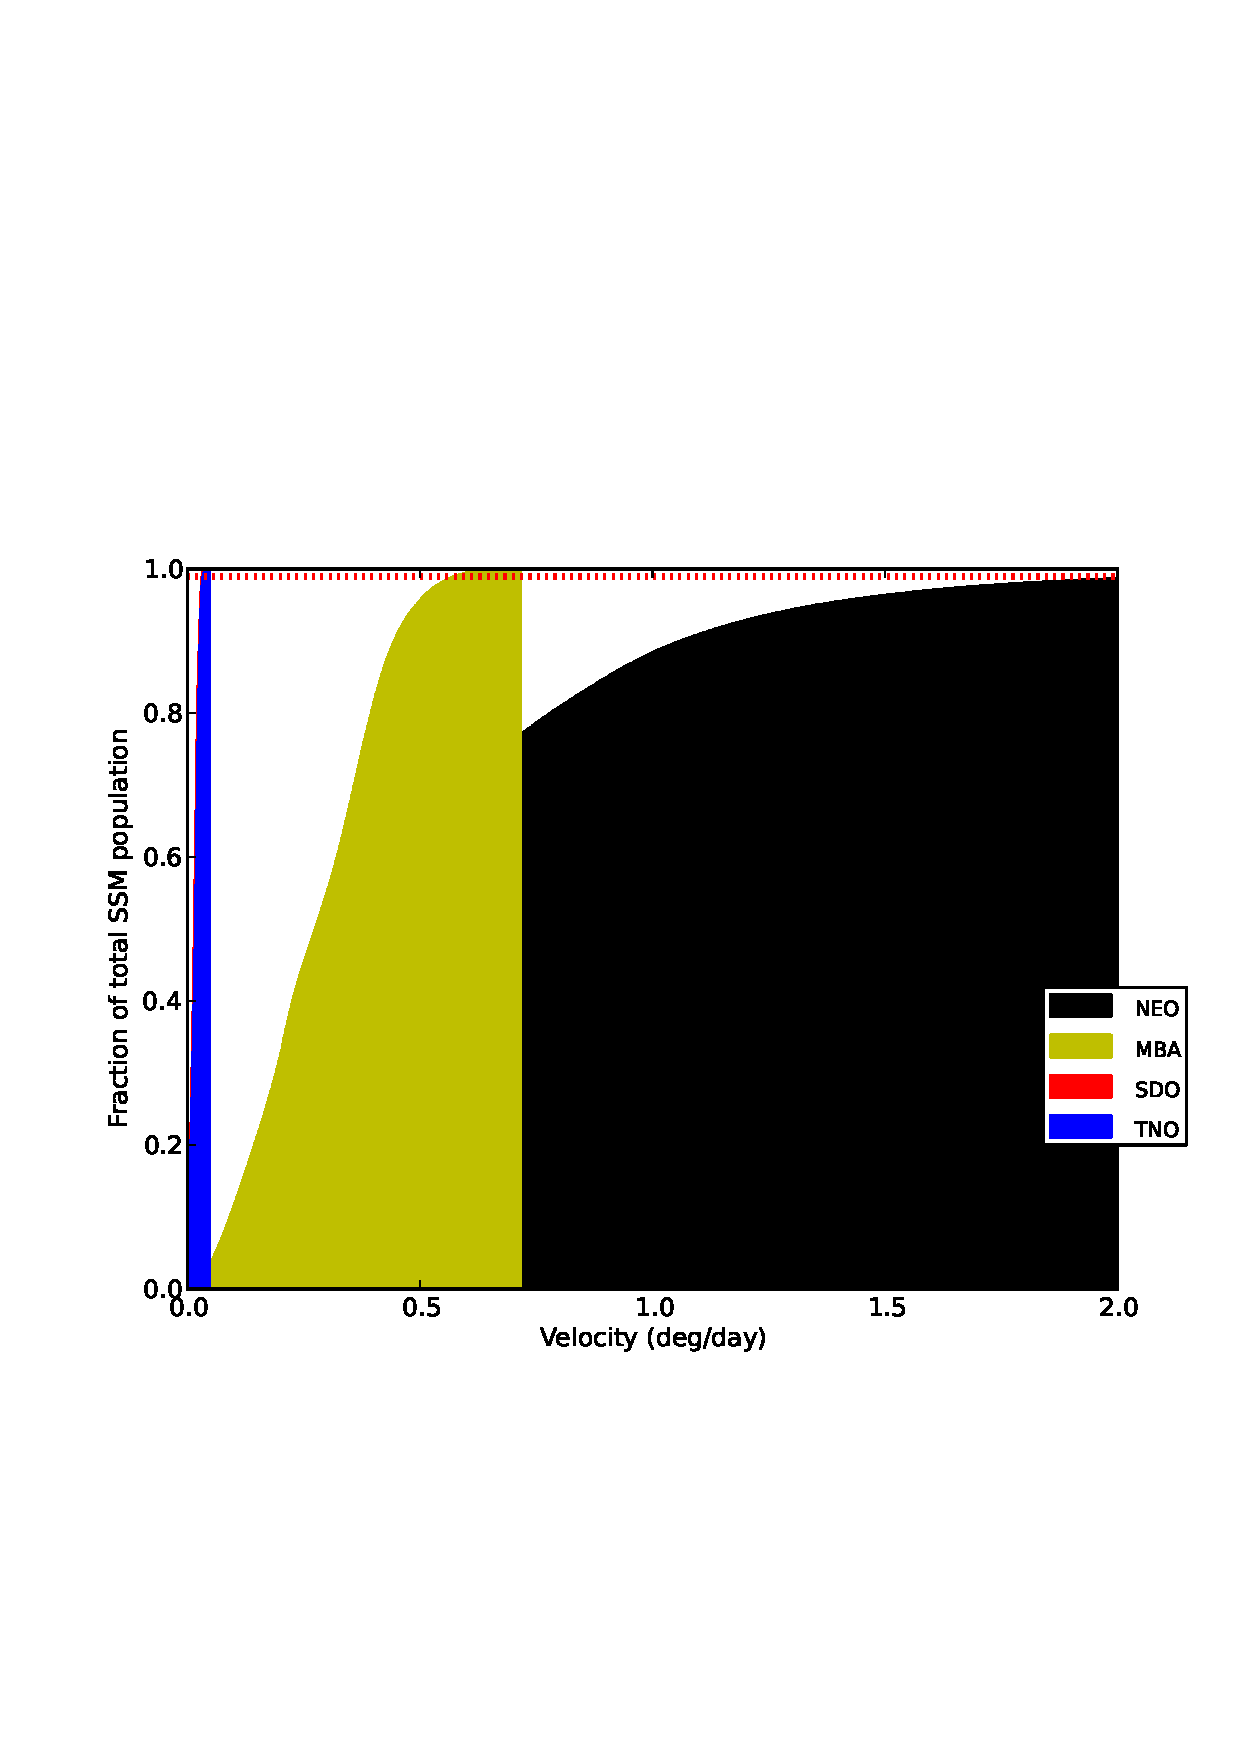
\includegraphics[width=13cm]{illustrations/mopsplots/aug2011/n_velocity.png}
  \caption{A cumulative histogram of solar solar system object
    sky-plane velocities, organized by classification.  Note that only
    the near-earth objects have higher velocities than main-belt
    asteroids.}
  \label{velSurvey}
\end{figure}

\begin{figure}[ht!]
  \centering
  \subfloat[Apparent Accelerations in Right Ascension over 15 Days]{
    \includegraphics[width=8cm]{illustrations/mopsplots/aug2011/n_accel_ra_15.png}
    }
  \subfloat[Apparent Accelerations in Right Ascension over 30 Days]{
    \includegraphics[width=8cm]{illustrations/mopsplots/aug2011/n_accel_ra_30.png}
    }

  \subfloat[Declination Apparent Accelerations in Declination over 15 Days]{
    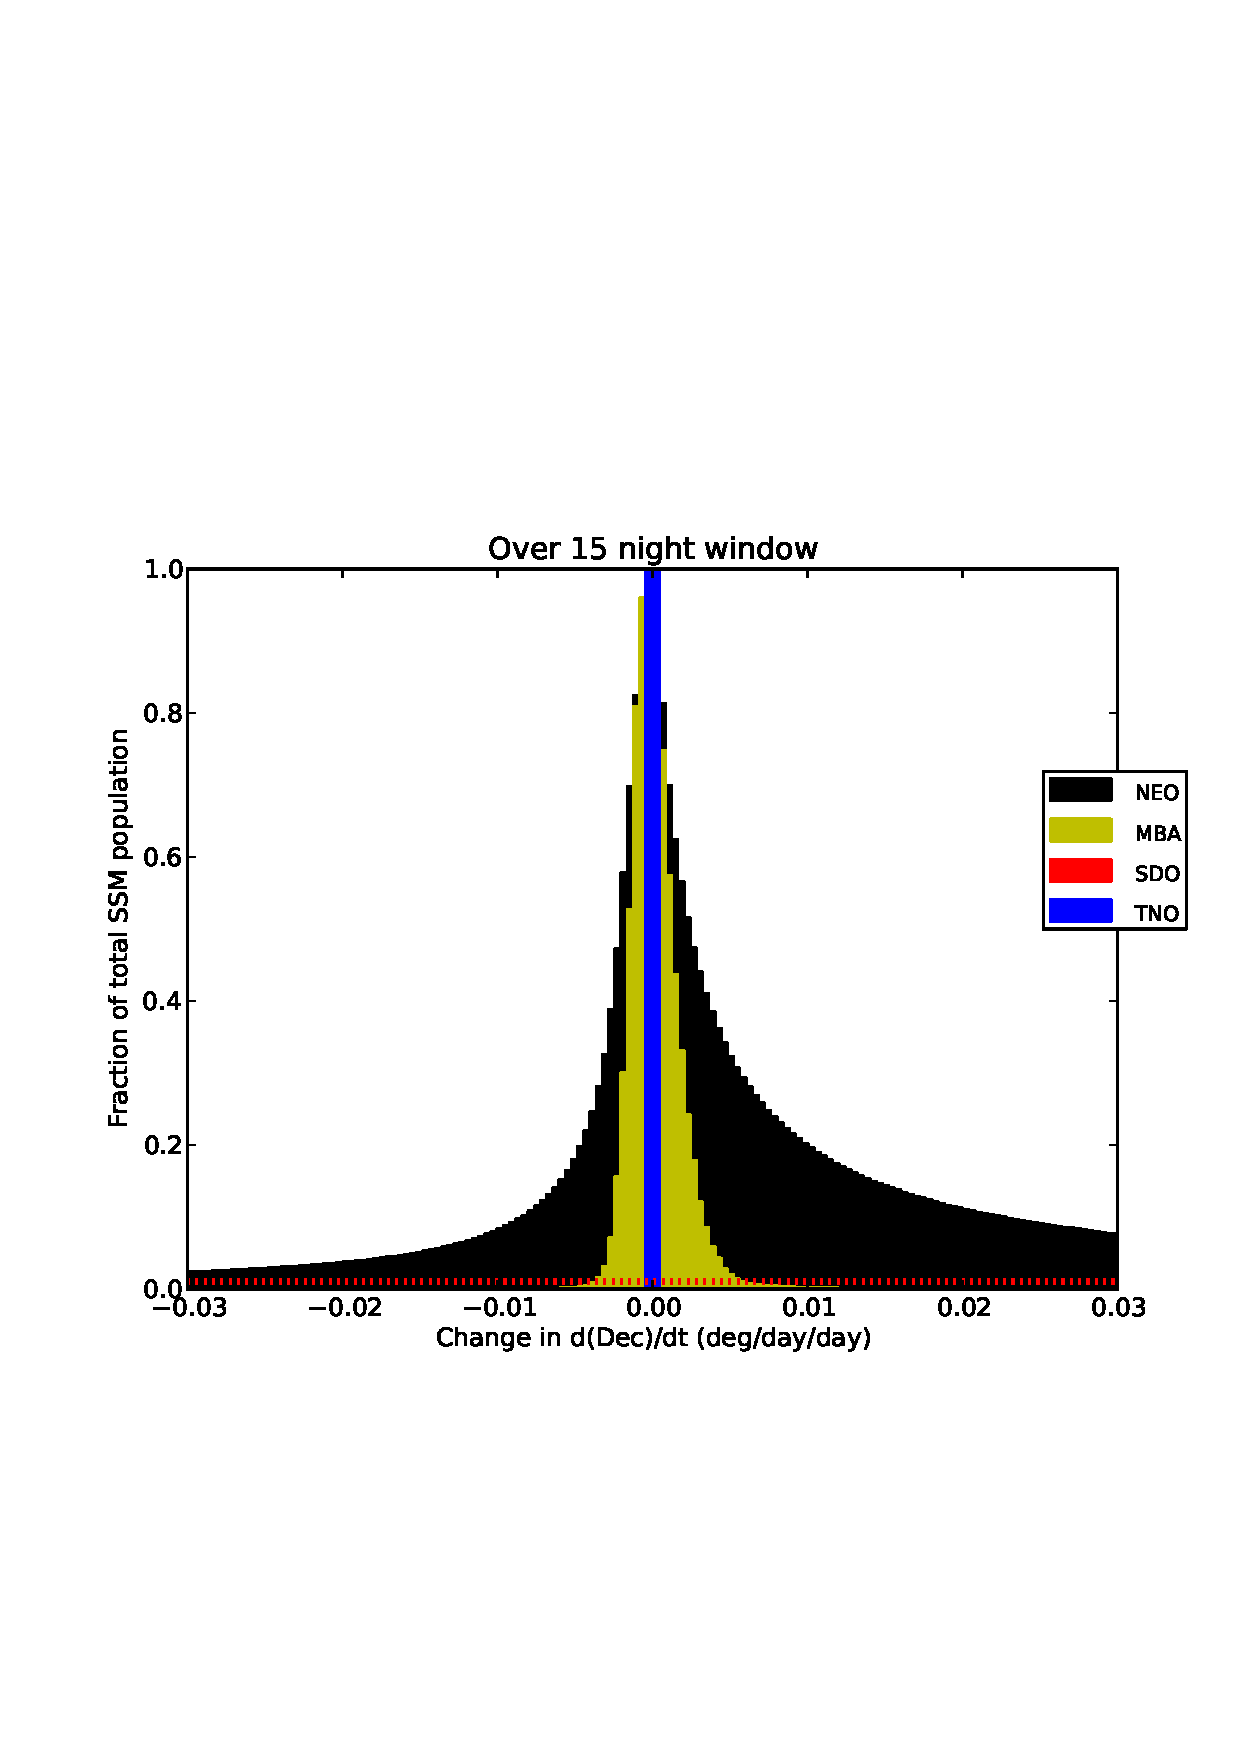
\includegraphics[width=8cm]{illustrations/mopsplots/aug2011/n_accel_dec_15.png}
    }
  \subfloat[Declination Apparent Accelerations in Declination over 30 Days]{
    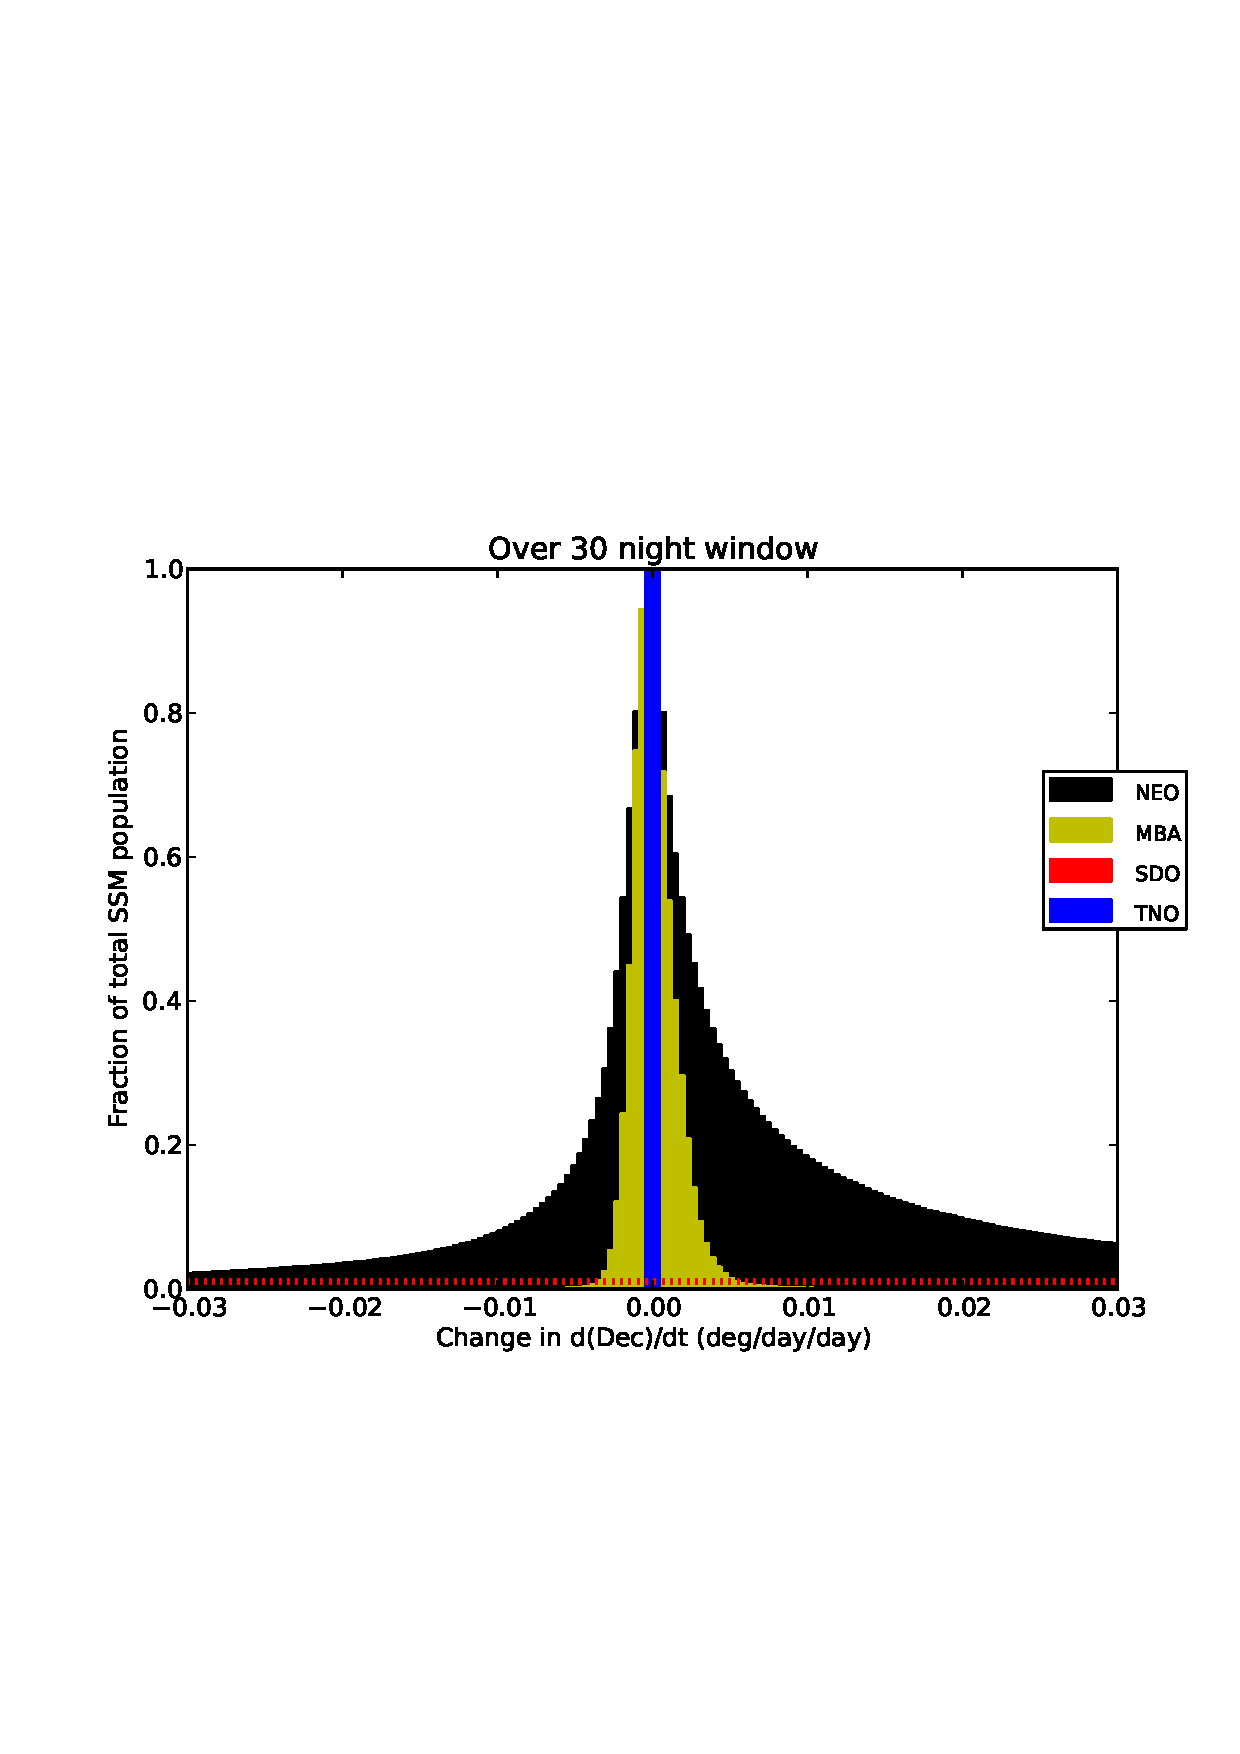
\includegraphics[width=8cm]{illustrations/mopsplots/aug2011/n_accel_dec_30.png}
    }
  \caption{Normalized histograms of sky-plane accelerations of several
    classes solar system objects in the RA and declination, with
    objects grouped by classification.  Histograms are presented for
    changes over 15 days and 30 days. The best-fit accelerations vary
    slightly given the size of the window; this is due to
    non-quadratic factors not included in the simple quadratic model.
    15 day tracking windows are used in the experiments presented in
    this document, but we expect to move to 30 day windows in the
    future.  In both cases, virtually all MBAs, and all other objects
    except NEOs, should have accelerations between -.02 and .02
    deg/day$^2$ in both axes.}
  \label{accSurvey}
\end{figure}


In order to determine reasonable limits on velocity and acceleration
of various classes of solar system objects, a survey of the solar
system model \citep{Grav2011} was conducted, see figures
\ref{velSurvey}, \ref{accSurvey} for histograms
presenting the results of these surveys.

We found that a velocity limit of .5 deg/day and an acceleration limit
.02 deg/day$^2$ would be generally sufficient.  By examining the
detections on an object-per-object basis, we calculated that among the
186,344 objects seen with proper cadence for OD, 186,209 of these
(more than 99.9\%) should generate useful tracks given these limits.

%% see mops64: /mnt/raid/jmyers/variousDensities/fullDensity/maxV.5_15days/trueTracks/*.log





\subsection{Results}

All simulations were conducted on the Gordon cluster at San Diego
Supercomputing Center.  Because of the large memory requirements for
running MOPS, the vSMP nodes were used for all stages of computation.
Except for the scaling tests, 16 threads were used for all the runs.


\begin{figure}[ht!]
\centering
\begin{tabular}{|r l|}
\hline
Number of asteroid detections: & 36,311,037 \\
Number of non-asteroid detections: & 0 \\
Average detections per night: & 1,134,719 \\
 & \\
Number of tracklets found: & 12,890,181 \\
Number of true tracklets: & 6,859,331 \\
Tracklets \% true: & 53.2\%\\
Tracklet generation time: & 4,791 sec (1.33 hours) \\
Tracklet generation memory use: & 13.7 GB  \\
 & \\
Number of tracks found: & 10,423,382 \\
Number of true tracks: & 5,779,424 \\
Track \% true: & 55.4\% \\
Track generation time: & 36,237 sec (10.1 hours) \\
Track generation memory use: & 16.2 GB \\
 & \\
Number of found objects: & 854,037 \\
Number of findable objects: & 1,128,643 \\
Found / findable: & 75.7\% \\
\hline
\end{tabular}

\caption{Results from the MOPS run without noise.  Velocity limit was .5 deg/day, acceleration limit was .02 deg/day$^2$ and the track chi squared probability limit was .9.  Note that not quite one fourth of objects which should generate plausible tracks are rejected.}
\label{oneMonth}
\end{figure}

\subsubsection{Survey Efficiency}
Figure~\ref{oneMonth} shows in-depth stats for a survey without noise.
As in all our runs, track generation is far more expensive than
tracklet generation in terms of CPU usage, but both require
substantial amounts of memory.  Also note that nearly one fourth of
the findable objects (those which should generate useful tracks) are
not found.  We expect that this is because of overly-aggressive
filtering in the chi squared probability filter.


\subsubsection{Nightly Variance in Runtime}

The cost of running MOPS depends on a variety of factors which are
largely dependent on telescope operations, such as revisit rates and
the locations of revisits.  Figure~\ref{nightlyVariance} shows some of
the 


\begin{figure}[ht!]
  \centering
  \subfloat{
    \includegraphics[width=12cm]{newIllustrations/tracklets_nightly.png}
    }
  \\
  \subfloat{
    \includegraphics[width=12cm]{newIllustrations/tracks_nightly.png}
    }

  \caption{Per-night costs of tracklet generation and track
    generation. Also, in the track generation section,
    note that because only 31 sets of nightly tracklets were
    generated, later runs had less data in their window and thus ran
    considerably faster.  This is an artifact of the experiment and
    not a meaningful trend.}
  \label{nightlyVariance}
\end{figure}


\subsubsection{Scaling on Non-Asteroid Sources}

Actual images will contain DiaSources from non-asteroid sources:
variable stars, supernova, and image processing artifacts (e.g. from
bright stars) will also be present.  Because the quality of image
processing is not known, we added non-asteroid ``noise'' detections to
images at varying rates.  At each rate, a fixed $n$ noise detections
were added to each image, with locations chosen at random.  We
successfully ran MOPS using densities as high as 5,000 non-asteroid
sources per image.  After adding 10,000 non-asteroid sources per
image, tracklet generation was possible but linking tracklets into
tracks was too slow - at over 48 hours for a single night of
searching, it exceeded the wall-clock limit on Gordon jobs.

Figure~\ref{noiseScaling_detections} shows some information about the
detection catalogs generated at each of the noise densities.  For each
of these catalogs, tracklet generation was performed for each of the
31 simulated nights of observation; results can be seen in
Figure~\ref{noiseScaling_tracklets}.  As expected, increasing numbers
of false detections lead to worse-than-linear increases in mislinkage.
This lead to worse-than-linear increases in computational costs for generating the
tracklets, both in terms of CPU and memory usage.

The tracklets generated in the tracklet generation test were used to
test scaling of track generation.  For reasons of time, we only
attempted to search for tracks starting on the first night of
observation.  Results are presented in
Figure~\ref{noiseScaling_tracks} and Figure~\ref{noiseScaling_found}.
The CPU time cost for track generation scaled worse-than-linearly on
the number of tracklets.  However, we saw only modest increases in the
number of output tracks and runtime for linkTracklets.  Also note that
the number of objects found remained nearly constant across the
various runs.



\begin{figure}[ht!]
\centering

\begin{tabular}{|c c c c|}
\hline
Per-Image Noise Density & Total number of detections & \% noise detections &  \\ 
0             & 36,311,037             & 0\%                          & \\
1,250         & 72,258,537             & 49.7\%          & \\
2,500         & 108,206,037            & 66.4\%          & \\ 
5,000         & 180,101,037            & 79.8\%          & \\
\hline
\end{tabular}
\caption{An overview of the detection sets used for the scaling tests on noise density.}
\label{noiseScaling_detections}
\end{figure}

\begin{figure}[ht!]
\centering

\subfloat[Number of tracklets generated at various noise density levels]
{\includegraphics[width=8cm]{newIllustrations/tracklet_num.png}}
\subfloat[Tracklet \% true at various noise density levels]
{\includegraphics[width=8cm]{newIllustrations/tracklet_true.png}}
\\
\subfloat[Tracklet generation runtimes at various noise density levels]
{\includegraphics[width=8cm]{newIllustrations/tracklet_runtime.png}}
\subfloat[Tracklet generation memory use at various noise density levels]
{\includegraphics[width=8cm]{newIllustrations/tracklet_mem.png}}

\caption{Tracklets generated at varying densities of non-asteroid
  ``noise'' sources, and corresponding compute costs.  Each data point
  represents 31 days of tracklet generation.  The same asteroid
  catalog was used for each simulation, but increasing numbers of
  ``noise'' sources were added in each simulation (see
  Figure~\ref{noiseScaling_detections}). Note that the number of
  tracklets generated, and the computational costs to find them,
  increase quickly as noise density increases. This is apparently due
  to the increase of mislinked ``false tracklets''. }
\label{noiseScaling_tracklets}
\end{figure}


\begin{figure}[ht!]
\centering

\subfloat[Number of tracks generated at various noise density levels]
{\includegraphics[width=8cm]{newIllustrations/track_num.png}}
\subfloat[Track \% true at various noise density levels]
{\includegraphics[width=8cm]{newIllustrations/track_true.png}}
\\
\subfloat[Track generation runtimes at various noise density levels]
{\includegraphics[width=8cm]{newIllustrations/track_runtime.png}}
\subfloat[Track generation memory use at various noise density levels]
{\includegraphics[width=8cm]{newIllustrations/track_mem.png}}

\caption{Tracks generated at varying densities of non-asteroid
  ``noise'' sources, and corresponding compute costs.  Detections
  catalogs with increasing numbers of noise detections
  (Figure~\ref{noiseScaling_detections}) and tracklets generated from
  these catalogs (Figure~\ref{noiseScaling_tracklets}) were used to generate
  linkTracklets input. For reasons of time, each linkTracklets run
  attempted to find only tracks which started on the first night of
  data and ended anywhere within the first 15 days.}
\label{noiseScaling_tracks}
\end{figure}


\begin{figure}[ht!]
\centering
\begin{tabular}{|c c c|}
\hline

Noise Density & Number of Tracklets & Found Objects \\
0 & 6,312,807 & 55,982 \\
1,250 & 13,318,186 & 55,870  \\
2,500 & 25,824,121 &  55,751  \\
5,000 & 66,635,397 &  55,464  \\
\hline
\end{tabular}

\caption{Objects found by linkTracklets with varying densities of
  noise in the input catalogs.  Note that the number of objects found
  is only slightly affected by the presence of noise in the input
  catalogs.}
\label{noiseScaling_found}
\end{figure}



\subsection{Conclusions}

For LSST images, we expect that 50-80\% of the DiaSources in our
catalogs will be attributable to non-asteroid sources.  This
corresponds to roughly 1250 or 5000 ``noise'' points per image, as we
simulated.

To meet requirements, we must be capable of running one night's-worth
of tracklet generation, track generation, and per-track IOD within 24
hours.  For the 50\% noise case, we saw a maximum tracklet generation
time of 10 minutes (using 16 CPUs) and for the 80\% noise case we saw
a maximum tracklet generation time of 21 minutes (again using 16
CPUs).  In our testing of track generation, we saw 306,866 tracks and
461,902 tracks generated in the 50\%-noise and 80\%-noise cases
respectively.  Expecting a trivially parallel IOD and an IOD cost of
roughly .001 seconds/track, we anticipate that IOD should not be
problematic: given a few hundred CPUs, we should be able to complete
the nightly IOD processing in a few wall-clock hours.

The cost of running linkTracklets, however, could be problematic given
the 24-hour limit.  As seen in Figure~\ref{noiseScaling_tracks},
linkTracklets can be quite slow, and runtimes can increase
worse-than-linearly on the number of input tracks, with non-linear
factors becoming significant somewhere between the 50\%-noise and
80\%-noise cases.  In the 50\%-noise experiment, runtime for a single
night was only 1.4 hours, but for the 80\%-noise experiment, runtime
was 32.5 hours!  Again, both experiments used 16 CPUs.  

In our one-month run of linkTracklets without noise, we found the
per-night cost of tracklet generation could vary by a factor of two or
more.  Applying this to the runs performed with noise, this gives us
an estimated maximum nightly runtime of between 2.8 and 65
hours (assuming 16 CPUs).

In order to reach the goal of running tracklet generation, track
generation, and IOD on the tracks, we should aim to reduce the maximum
runtime of linkTracklets to below 20 hours in the worst case.  This
requires a speedup of roughly 3-4 over the current performance.  Such
a speedup may be possible simply by waiting on Moore's law, but to be
safe it would be preferable to begin aggressively experimenting with
larger numbers of threads and possible sequential optimizations as
soon as possible.  

Preliminary scaling experiments showed little additional speedup when
using more than 16 CPUs, and a possible slowdown as the number of CPUs
exceeded 20.  However, these tests were conducted using a smallish
data set, and should be repeated with a larger one.  Initial tests
were also conducted on Gordon vSMP nodes, which hold only 16 CPUs per
motherboard; this is another possible cause of the poor scaling beyond
16 CPUs, and should be compared with scaling tests on conventional
single-board, large-memory UMA machines.


\section{Implications for Survey Performance}
% tbd: expand this into its own file...
Talk here about OpSim, cadence, software limitations and science requirements.

\section{Risk Reduction}

Though the core algorithms of MOPS have been implemented in
LSST-appropriate style, further research and development are needed.



\subsection{Long Duration Survey Performance}

Current simulations cover fairly short time periods, and therefore
emphasize the problem of initial object discovery.  In the course of
the full survey, we expect that many detected sources will be
attributed to already-discovered objects.  Because initial object
discovery phases are relatively expensive and ephemeris calculation is
relatively fast, we expect that the resource usage of the system will
decline over time, as more objects are discovered and the size of
input catalogs is reduced.  This expectation needs to be verified and
quantified.

Attribution, precovery and Moving Object management and refinement of the
Moving Object table are not yet implemented in LSST-compliant software.
Developing this software should be a significant development task.
However, we hope that by using the algorithms from the PanSTARRS MOPS
we can avoid any significant research tasks.

To test this software, we will need to generate simulated input
catalogs which span longer time periods.  Accomplishing this will
require either significant compute-resources or improved tools for
generating input catalogs.


\subsection{Future Software Development Tasks}

\subsubsection{Filtering on Trailing for Near-Earth-Object Searching}

\label{neosTrailing}

Near-Earth Objects tend to have the highest sky-plane velocity.  This
presents a significant challenge; as we increase the maximum velocity
limit of our tracklet generation, the potential for mislinkage
increases significantly, leading to higher numbers of tracklets and
increased costs.  

Fortunately, fast-moving NEOs will generate visible trails in our
images.  By requiring all tracklets to show trails consistent with
their apparent sky-plane velocity, we expect that it will be possible
to filter most false tracklet linkages, thus rendering the problem of
NEO searching manageable.

The ability to filter on trailing is dependent almost entirely on our
ability to correctly identify trails in images.  Currently, the
ability of image processing to detect trails is not well quantified.  To
remedy this, we will need to generate simulated images which include
asteroid trails and send them to image processing; further refinement
of image processing algorithms may be neccesary.



\subsubsection{Distribution/Parallelization of Software}
\label{parallelization}

To meet the needs of full operations, DayMOPS will almost certainly
need to utilize some form of parallelism in order to reduce runtime.
For some components, such as orbit determination, this should be
easily achieved; others will require closer attention to detail.  We
have planned parallel or distributed versions for most components,
which are described below.  In some cases we have also experimented
with various initial implementations, which are noted.

%% do we need this?
%% \subsubsubsection{Tools And Methods}
%% \paragraph{Multithreading and OpenMP}
%% \paragraph{Distributed Shared Memory}
%% \paragraph{Full Distribution and MPI}


\subsubsubsection{Orbit Determination} Orbit Determination is
performed per-track; we expect that it will be slow only because the
number of tracks will be very large.  Thus, we expect that Orbit
Determination should be trivially parallel; simply divide the tracks
between various machines or CPU cores. 

\subsubsubsection{Parallel FindTracklets} The findTracklets section of
our pipeline tends to run very quickly.  For this reason, we do not
anticipate that parallelizing findTracklets will be necessary at all.
However, if we choose to parallelize it, then it should be trivial to
distribute the workload; one query is performed per input detection,
and each query is naturally independent, so it should be trivial to
parallelize the work at this level.  This could be accomplished by
changing the outer ``for'' loop to a ``parallel for'' loop, e.g. using
OpenMP.  We anticipate that the detections as well as the trees over
detections should fit in memory, making explicit distribution
unnecessary.

\subsubsubsection{Parallel CollapseTracklets} It has been our
experience that the collapseTracklets phase is generally quite fast,
and will likely not need parallelization.  One tree query will be
performed per tracklet, which provides a natural axis of parallelism.
However, there is potential for some contention between CPUs as we
normally check whether an input tracklet has been collapsed already by
a prior query, and if so, do not attempt to work with it.  Dealing
with this conditional will require synchronization between CPUs, which
could hamper performance.  It might also be ignored, perhaps allowing
the redundant work to happen in order to avoid the synchronization
costs.

\subsubsubsection{Parallel LinkTracklets} We have experimented with a
parallel, shared-memory linkTracklets implementation based on OpenMP.
The linkTracklets phase creates a tree of tracklets at each image
which generated tracklets, and attempts searching using each
temporally well-separated pair of trees as endpoint trees, with
intermediate-time trees as sources of possible support.  Each of these
searches is independent, so this provides a fairly natural axis of
parallelism.  However, this does not address the potential case where
the trees become larger than memory, which we have determined to be a
plausible problem.  To deal with this, we have used the kernel-level
distributed shared-memory provided by vSMP on the Dash and Gordon
clusters.  This way, a series of distributed machines provide the
appearance of a shared-memory system for OpenMP.  It may also be
possible to accomplish a similar effect by explicitly rewriting
linkTracklets to use a user-level distributed shared memory library
and MPI.  

\subsubsubsection{Distributed LinkTracklets} In case the implicit
memory sharing is not sufficient, it may be necessary to write an
explicitly distributed linkTracklets.  This was attempted by a CS
Master's student, Matt Cleveland, working with Prof. Dave Lowenthal.
The design was well-thought out but complex, leading to slow
implementation.  The distributed version was forked off before a
variety of changes to the serial version were made, and never merged
back.

The distributed linkTracklets held only the higher levels of trees and
the tracklets of the endpoint trees on the master node.  The master
node would attempt the linking algorithm on the higher levels of the
tree until it reached a terminal point; it would then attempt to
predict the amount of work needed to complete the linking and save the
state of the searching and estimated cost to a buffer.  Periodically,
the work items in the buffer are distributed to worker nodes, with
attention given to load distribution as well as cache issues,
attempting to minimize the amount of data which must be transferred to
worker nodes.


\subsubsubsection{Parallel Subset Removal}


\appendix
\section{Helpful Metrics and Software Tools}
\subsection{Studying OpSim}
\subsection{Studying Tracks}




% so jeff larsen gave me a list of references as \bibitems.  our other
% references are bibtex format.  So we now have two bibliographies!
% ugly! hopefully no one will particularly care.
\begin{thebibliography}{99}

%% These came from Jeff Larsen for his intro section
\bibitem[Bode(1802)]{1802QB378} Bode, J.~E.\ 1802, Berlin : In 
der Himburgischen Buchhandlung, 1802.

\bibitem[Chiang and Brown (1999)]{MB} {Chiang}, E.~I. and {Brown}, M.~E. 1999,
      \aj, 118, 1411

\bibitem[Gehrels et al.(1990)]{1990ASPC....8...51G} Gehrels, T., McMillan, 
R.~S., Scotti, J.~V., \& Perry, M.~L.\ 1990, CCDs in astronomy, 8, 51 

\bibitem[Gladman et al. (1998)]{BG} {Gladman}, B. and {Kavelaars}, J.~J.
      and {Nicholson}, P.~D. and {Loredo}, T.~J. and {Burns}, J.~A. 1998, \aj,
      116, 2042

\bibitem[Gural et al.(2005)]{2005AJ....130.1951G} Gural, P.~S., Larsen, 
J.~A., \& Gleason, A.~E.\ 2005, \aj, 130, 1951 

\bibitem[Larson(2007)]{2007IAUS..236..323L} Larson, S.\ 2007, IAU 
Symposium, 236, 323 

\bibitem[Pravdo et al.(1999)]{1999AJ....117.1616P} Pravdo, S.~H., 
Rabinowitz, D.~L., Helin, E.~F., et al.\ 1999, \aj, 117, 1616 

\bibitem[Rabinowitz(1991)]{1991AJ....101.1518R} Rabinowitz, D.~L.\ 1991, 
\aj, 101, 1518 

\bibitem[Shoemaker 
\& Shoemaker(1988)]{1988NASTM4041...52S} Shoemaker, C.~S., \& Shoemaker, E.~M.\ 1988, NASA Tech.~Memo., NASA TM-4041, p.~52 - 54, 4041, 52 

\bibitem[Stokes et al.(2000)]{2000Icar..148...21S} Stokes, G.~H., Evans, 
J.~B., Viggh, H.~E.~M., Shelly, F.~C., \& Pearce, E.~C.\ 2000, \icarus, 148, 21 

\bibitem[Tombaugh(1960)]{1960S&T....19..264T} Tombaugh, C.~W.\ 1960, \skytel, 19, 264 

\bibitem[van Houten et 
al.(1970)]{1970A&AS....2..339V} van Houten, C.~J., van Houten-Groeneveld, I., Herget, P., \& Gehrels, T.\ 1970, \aaps, 2, 339 

\bibitem[Wolf(1892)]{1892AN} Wolf, M.\ 1892, Astronomische 
Nachrichten, 129, 337 

\end{thebibliography}

\bibliographystyle{apj}
\bibliography{baseline}




\end{document}
